\subsection{Bearing walls}

\begin{figure}
  \begin{center}
  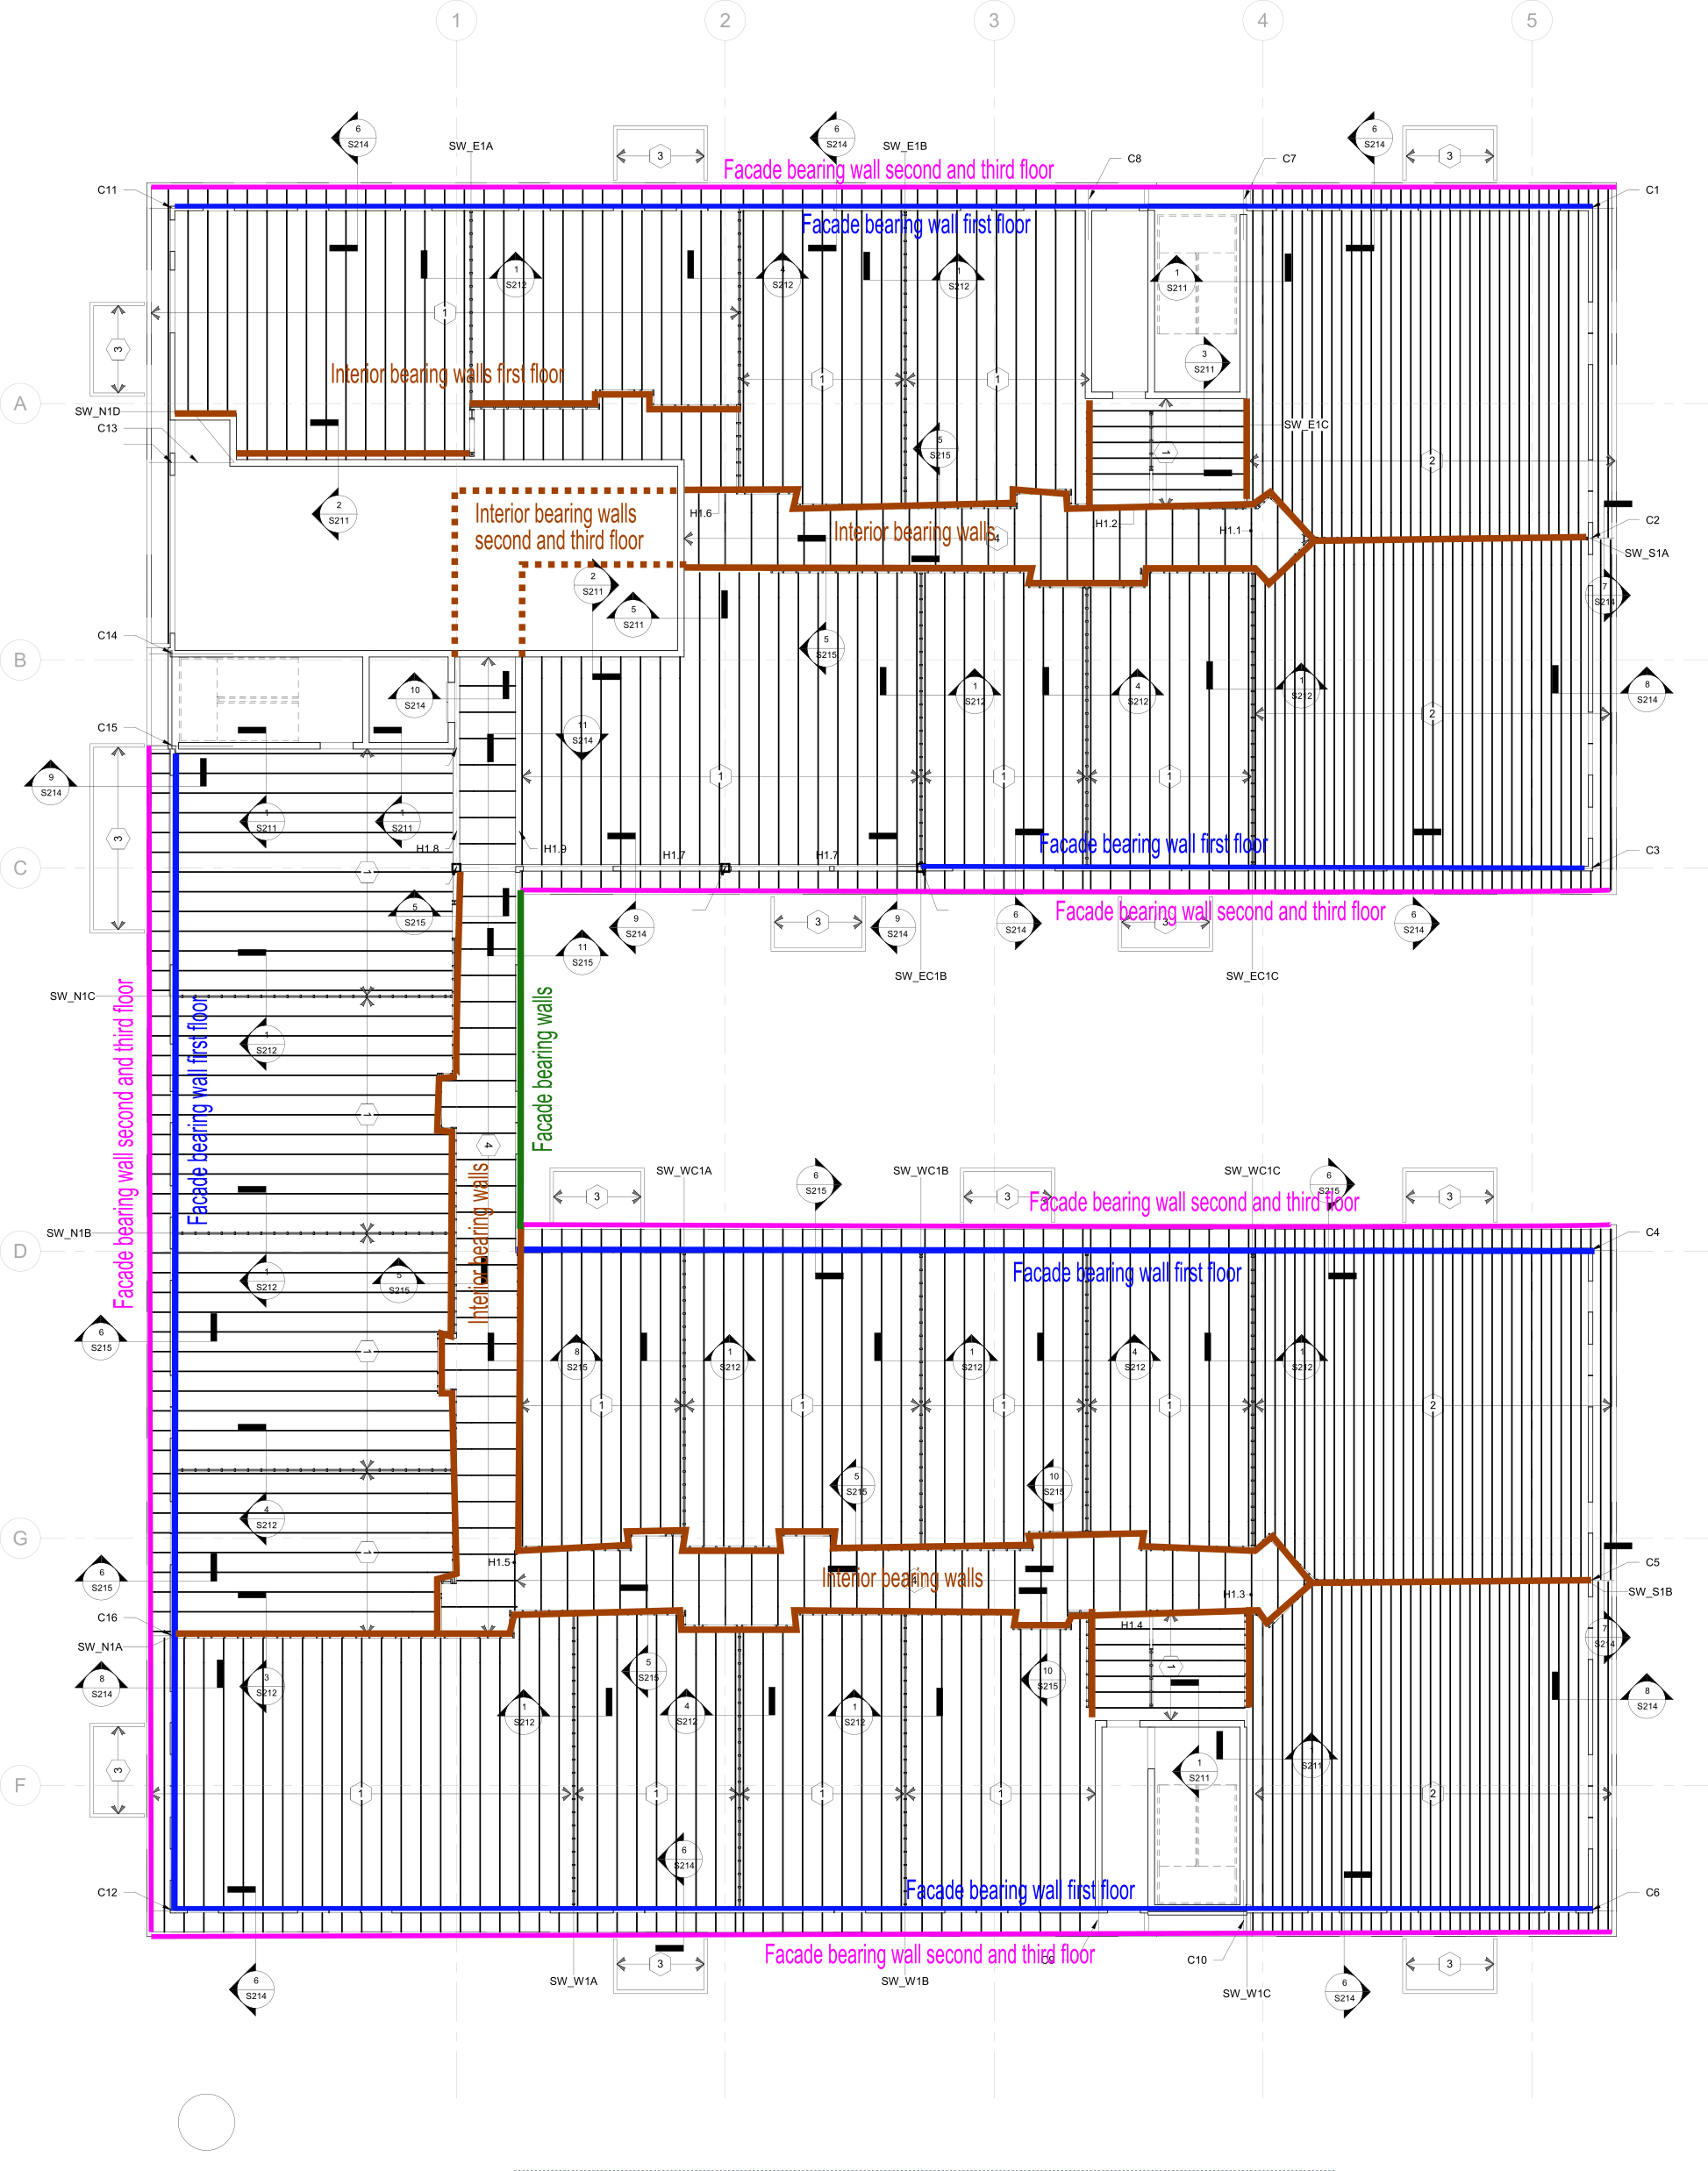
\includegraphics[width=120mm]{figures/bearing_walls_key_plan}
  \end{center}
  \caption{Bearing walls key plan. Roof}\label{fg_bearing_walls_key_plan}
\end{figure}

\subsubsection{Facade bearing walls at first floor}

\paragraph{Loads.}

\begin{itemize}
\item Vertical load: 43.34 kN/m
\item Vertical load on each stud: 21.14 kN
\item Wind load on stud height: 0.42 kN/m
\end{itemize}

\paragraph{Internal forces.}

\noindent Internal forces:

\begin{align}
  N_{max}&= 21.14\ kN \\
  M_{max}&= 0.36\ kN \cdot m
\end{align}

\paragraph{Bending and axial compression check.}

\subparagraph{Mechanical properties}

\begin{itemize}
\item Species: Hem-fir stud
\item Spacing: $0.49\ m$
\item Stud height: 2.64 m
\item Repetitive member factor: $C_r= 1.15$
\item Size factor: $C_F= 1.3$
\item $E_{min}= 3.03\ GPa$
\item $F'_c= 6.09\ MPa$.
\item $F'_b= 6.97\ MPa$.
\item Sections dimensions: (2x8''), effective (1.5x7.5'')= $38.1 \times 190.5\ mm$.
\item Unbraced length x axis: 2.64 m
\item Unbraced length y axis: 0.3 m
\item Stud stability factor: $C_P= 0.85$
\end{itemize}

\begin{equation}
  N'_s= 44.21\ kN
\end{equation}

\noindent Capacity factor according to section 3.9.2 of NDS-2018 (equations 3.9.3 and 3.9.4):

\begin{equation}
  CF= 0.52 < 1 \implies OK
\end{equation}

\subsubsection{Facade bearing walls at second floor}

\paragraph{Loads.}

\begin{itemize}
\item Vertical load: 30.52 kN/m
\item Vertical load on each stud: 14.88 kN
\item Wind load on stud height: 0.42 kN/m
\end{itemize}

\paragraph{Internal forces.}

\noindent Internal forces:

\begin{align}
  N_{max}&= 14.88\ kN \\
  M_{max}&= 0.36\ kN \cdot m
\end{align}

\paragraph{Bending and axial compression check.}

\subparagraph{Mechanical properties}

\begin{itemize}
\item Species: Hem-fir stud
\item Spacing: $0.49\ m$
\item Stud height: 2.64 m
\item Repetitive member factor: $C_r= 1.15$
\item Size factor: $C_F= 1.3$
\item $E_{min}= 3.03\ GPa$
\item $F'_c= 6.09\ MPa$.
\item $F'_b= 6.95\ MPa$.
\item Sections dimensions: (2x8''), effective (1.5x7.5'')= $38.1 \times 190.5\ mm$.
\item Unbraced length x axis: 2.64 m
\item Unbraced length y axis: 0.3 m
\item Stud stability factor: $C_P= 0.85$
\end{itemize}

\begin{equation}
  N'_s= 44.21\ kN
\end{equation}

\noindent Capacity factor according to section 3.9.2 of NDS-2018 (equations 3.9.3 and 3.9.4):

\begin{equation}
  CF= 0.38 < 1 \implies OK
\end{equation}

\subsubsection{Facade bearing walls at third floor}

\paragraph{Loads.}

\begin{itemize}
\item Vertical load: 16.01 kN/m
\item Vertical load on each stud: 7.81 kN
\item Wind load on stud height: 0.42 kN/m
\end{itemize}

\paragraph{Internal forces.}

\noindent Internal forces:

\begin{align}
  N_{max}&= 7.81\ kN \\
  M_{max}&= 0.36\ kN \cdot m
\end{align}

\paragraph{Bending and axial compression check.}

\subparagraph{Mechanical properties}

\begin{itemize}
\item Species: Hem-fir stud
\item Spacing: $0.49\ m$
\item Stud height: 2.64 m
\item Repetitive member factor: $C_r= 1.15$
\item Size factor: $C_F= 1.3$
\item $E_{min}= 3.03\ GPa$
\item $F'_c= 6.09\ MPa$.
\item $F'_b= 6.96\ MPa$.
\item Sections dimensions: (2x8''), effective (1.5x7.5'')= $38.1 \times 190.5\ mm$.
\item Unbraced length x axis: 2.64 m
\item Unbraced length y axis: 0.3 m
\item Stud stability factor: $C_P= 0.85$
\end{itemize}

\begin{equation}
  N'_s= 44.21\ kN
\end{equation}

\noindent Capacity factor according to section 3.9.2 of NDS-2018 (equations 3.9.3 and 3.9.4):

\begin{equation}
  CF= 0.28 < 1 \implies OK
\end{equation}

\subsubsection{Top plates}

\paragraph{Loads}

\begin{itemize}
\item Load from trusses: 9.64 kN/truss.
\item Truss spacing: 0.61 m
\item Stud spacing: 0.49 m
\end{itemize}

\paragraph{Bending strength checking:}

\noindent Maximum induced moment:
\begin{align}
  M_{max}&= 0.42 kN \cdot m\\
  \sigma_{max}&= 9.21\ MPa
\end{align}

\noindent Bending strength:

\begin{equation}
  F'_b= 10.05\ MPa
\end{equation}

\noindent Structural bending check:

\begin{equation}
F'_b = 10.05 > 9.21 = \sigma_{max} \implies OK
\end{equation}

\paragraph{Perpendicular to grain strength checking:}

\noindent Maximum induced reaction:
\begin{align}
  R_{max}&= 9.38\ kN\\
  \sigma_{max,perp}&= 1.29\ MPa
\end{align}

\begin{equation}
F'_{c,perp} = 2.79 > 1.29 = \sigma_{max,perp} \implies OK
\end{equation}

\subsubsection{Interior bearing walls at first floor}

\paragraph{Loads.}

\begin{itemize}
\item Vertical load: 84.99 kN/m
\item Vertical load on each stud: 25.9 kN
\item Wind load on stud height: 0.0 kN/m
\end{itemize}

\paragraph{Internal forces.}

\noindent Internal forces:

\begin{align}
  N_{max}&= 25.9\ kN \\
  M_{max}&= 0.0\ kN \cdot m
\end{align}

\paragraph{Bending and axial compression check.}

\subparagraph{Mechanical properties}

\begin{itemize}
\item Species: Hem-fir stud
\item Spacing: $0.30\ m$
\item Stud height: 2.64 m
\item Repetitive member factor: $C_r= 1.15$
\item Size factor: $C_F= 1.3$
\item $E_{min}= 3.03\ GPa$
\item $F'_c= 4.89\ MPa$.
\item $F'_b= 6.96\ MPa$.
\item Sections dimensions: (2x6''), effective (1.5x5.5'')= 38.1 x 139.7  mm.
\item Unbraced length x axis: 2.64 m
\item Unbraced length y axis: 0.3 m
\item Stud stability factor: $C_P= 0.68$
\end{itemize}

\begin{equation}
  N'_s= 26.00\ kN
\end{equation}

\noindent Capacity factor according to section 3.9.2 of NDS-2018 (equations 3.9.3 and 3.9.4):

\begin{equation}
  CF= 0.99 < 1 \implies OK
\end{equation}

\subsubsection{Interior bearing walls at second floor}

\paragraph{Loads.}

\begin{itemize}
\item Vertical load: 59.93 kN/m
\item Vertical load on each stud: 18.26 kN
\item Wind load on stud height: 0.0 kN/m
\end{itemize}

\paragraph{Internal forces.}

\noindent Internal forces:

\begin{align}
  N_{max}&= 18.26\ kN \\
  M_{max}&= 0.0\ kN \cdot m
\end{align}

\paragraph{Bending and axial compression check.}

\subparagraph{Mechanical properties}

\begin{itemize}
\item Species: Hem-fir stud
\item Spacing: $0.30\ m$
\item Stud height: 2.64 m
\item Repetitive member factor: $C_r= 1.15$
\item Size factor: $C_F= 1.3$
\item $E_{min}= 3.03\ GPa$
\item $F'_c= 4.89\ MPa$.
\item $F'_b= 6.96\ MPa$.
\item Sections dimensions: (2x6''), effective (1.5x5.5'')= 38.1 x 139.7  mm.
\item Unbraced length x axis: 2.64 m
\item Unbraced length y axis: 0.3 m
\item Stud stability factor: $C_P= 0.68$
\end{itemize}

\begin{equation}
  N'_s= 26.00\ kN
\end{equation}

\noindent Capacity factor according to section 3.9.2 of NDS-2018 (equations 3.9.3 and 3.9.4):

\begin{equation}
  CF= 0.49 < 1 \implies OK
\end{equation}

\subsubsection{Interior bearing walls at third floor}

\paragraph{Loads.}

\begin{itemize}
\item Vertical load: 33.7 kN/m
\item Vertical load on each stud: 20.54 kN
\item Wind load on stud height: 0.0 kN/m
\end{itemize}

\paragraph{Internal forces.}

\noindent Internal forces:

\begin{align}
  N_{max}&= 20.54\ kN \\
  M_{max}&= 0.00\ kN \cdot m
\end{align}

\paragraph{Bending and axial compression check.}

\subparagraph{Mechanical properties}

\begin{itemize}
\item Species: Hem-fir stud
\item Spacing: $0.61\ m$
\item Stud height: 2.64 m
\item Repetitive member factor: $C_r= 1.15$
\item Size factor: $C_F= 1.3$
\item $E_{min}= 3.03\ GPa$
\item $F'_c= 4.89\ MPa$.
\item $F'_b= 6.96\ MPa$.
\item Sections dimensions: (2x6''), effective (1.5x5.5'')= 38.1 x 139.7  mm.
\item Unbraced length x axis: 2.64 m
\item Unbraced length y axis: 0.3 m
\item Stud stability factor: $C_P= 0.68$
\end{itemize}

\begin{equation}
  N'_s= 26.00\ kN
\end{equation}

\noindent Capacity factor according to section 3.9.2 of NDS-2018 (equations 3.9.3 and 3.9.4):

\begin{equation}
  CF= 0.62 < 1 \implies OK
\end{equation}

\subsubsection{Top plates}

\paragraph{Loads}

\begin{itemize}
\item Load from trusses: 11.81 kN/truss.
\item Truss spacing: 0.61 m
\item Stud spacing: 0.49 m
\end{itemize}

\paragraph{Bending strength checking:}

\noindent Maximum induced moment:
\begin{align}
  M_{max}&= 0.24 kN \cdot m\\
  \sigma_{max}&= 7.15\ MPa
\end{align}

\noindent Bending strength:

\begin{equation}
  F'_b= 10.05\ MPa
\end{equation}

\noindent Structural bending check:

\begin{equation}
F'_b = 10.05 > 7.15 = \sigma_{max} \implies OK
\end{equation}

\paragraph{Perpendicular to grain strength checking:}

\noindent Maximum induced reaction:
\begin{align}
  R_{max}&= 8.56\ kN\\
  \sigma_{max,perp}&= 1.61\ MPa
\end{align}

\begin{equation}
F'_{c,perp} = 2.79 > 1.61 = \sigma_{max,perp} \implies OK
\end{equation}
